% Supplementary material for anonymous ACCV submission.
\documentclass[runningheads]{llncs}
\usepackage{graphicx}
\usepackage{amsmath,amssymb}
\usepackage{color}
\usepackage{float}

\renewcommand{\thetable}{S\arabic{table}}
\renewcommand{\thefigure}{S\arabic{figure}}
\setlength{\textfloatsep}{6pt}
\setlength{\intextsep}{6pt}
\setlength{\floatsep}{6pt}

\begin{document}
\pagestyle{headings}
\mainmatter

\def\ACCVSubNumber{***}

\title{TriPoseFusion: Robust Multi-View 3D Driver Pose Fusion with Outlier-Aware Canonicalization\\
Supplementary Material}
\titlerunning{ACCV submission ID \ACCVSubNumber}
\authorrunning{ACCV submission ID \ACCVSubNumber}
\author{Anonymous ACCV Submission}
\institute{Paper ID \ACCVSubNumber}
\maketitle

\section{Environment-Wise Results}

Table~\ref{tab:supp_env_pose} reports the environment-wise comparison that is summarized in the main paper. TriPoseFusion remains below both the raw best-single and canonicalized best-single baselines in all four illumination settings.

\begin{table}[H]
\centering
\caption{Environment-wise comparison against raw and canonicalized best-single baselines. Values are averaged across 22 sequences per environment.}
\label{tab:supp_env_pose}
\scriptsize
\setlength{\tabcolsep}{2pt}
\begin{tabular}{lcccc}
\hline
Environment & Best raw (m) $\downarrow$ & Best canon. (m) $\downarrow$ & TriPoseFusion (m) $\downarrow$ & $\Delta$ vs canon. (m) \\
\hline
Day high & 1.971 & 0.806 & \textbf{0.435} & -0.371 \\
Day low & 2.284 & 1.133 & \textbf{0.391} & -0.742 \\
Night high & 1.976 & 0.833 & \textbf{0.418} & -0.415 \\
Night low & 2.081 & 0.936 & \textbf{0.417} & -0.519 \\
\hline
\end{tabular}
\end{table}

\begin{figure}[H]
\centering
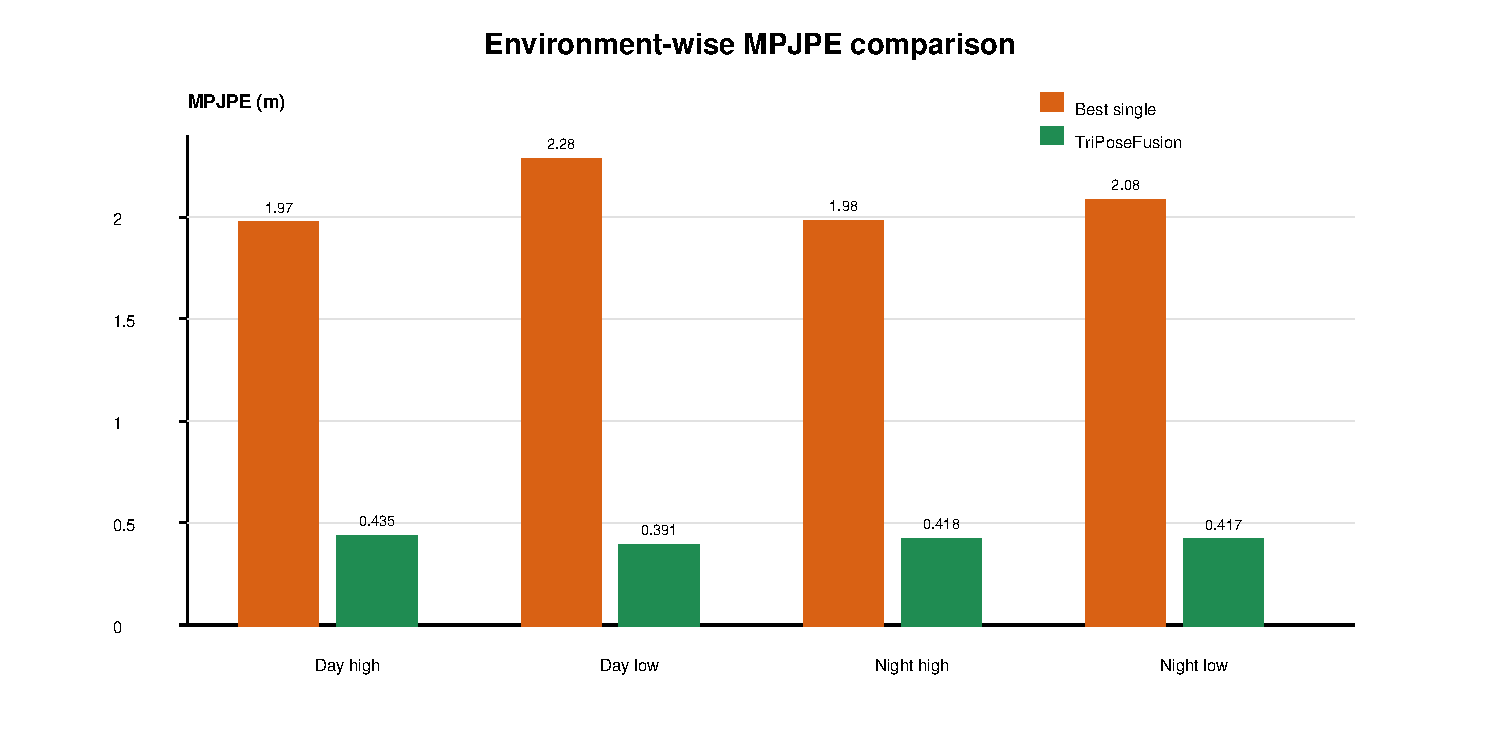
\includegraphics[width=0.72\linewidth]{figures/fig_environment_mpjpe.pdf}
\caption{Environment-wise MPJPE comparison. The plot visualizes the same environment-level trend as Table~\ref{tab:supp_env_pose}.}
\label{fig:supp_environment_mpjpe}
\end{figure}

\section{Additional Single-View Diagnostics}

Table~\ref{tab:supp_paired_single} reports a paired comparison between TriPoseFusion and an oracle best-single-view baseline over the 88 matched subject-environment pairs. The best-single baseline selects the lowest-error raw single camera for each sequence under the evaluation reference, so it is a diagnostic upper bound for fixed single-camera selection rather than a deployable method. TriPoseFusion improves MPJPE and PCK@0.10 on every matched pair. The smaller PA-MPJPE win count reflects that Procrustes alignment can remove global similarity differences from single-view predictions, so PA-MPJPE should be interpreted together with MPJPE and PCK.

\begin{table}[H]
\centering
\caption{Paired comparison against the raw oracle best-single-view baseline over 88 matched subject-environment pairs. Delta is TriPoseFusion minus best-single; lower is better for MPJPE/PA-MPJPE and higher is better for PCK.}
\label{tab:supp_paired_single}
\scriptsize
\setlength{\tabcolsep}{5pt}
\begin{tabular}{lcc}
\hline
Metric & Mean delta & TriPoseFusion better pairs \\
\hline
MPJPE (m) $\downarrow$ & -1.224 & 88 / 88 \\
PA-MPJPE (m) $\downarrow$ & -0.426 & 29 / 88 \\
PCK@0.10 $\uparrow$ & +0.139 & 88 / 88 \\
\hline
\end{tabular}
\end{table}

\begin{figure}[H]
\centering
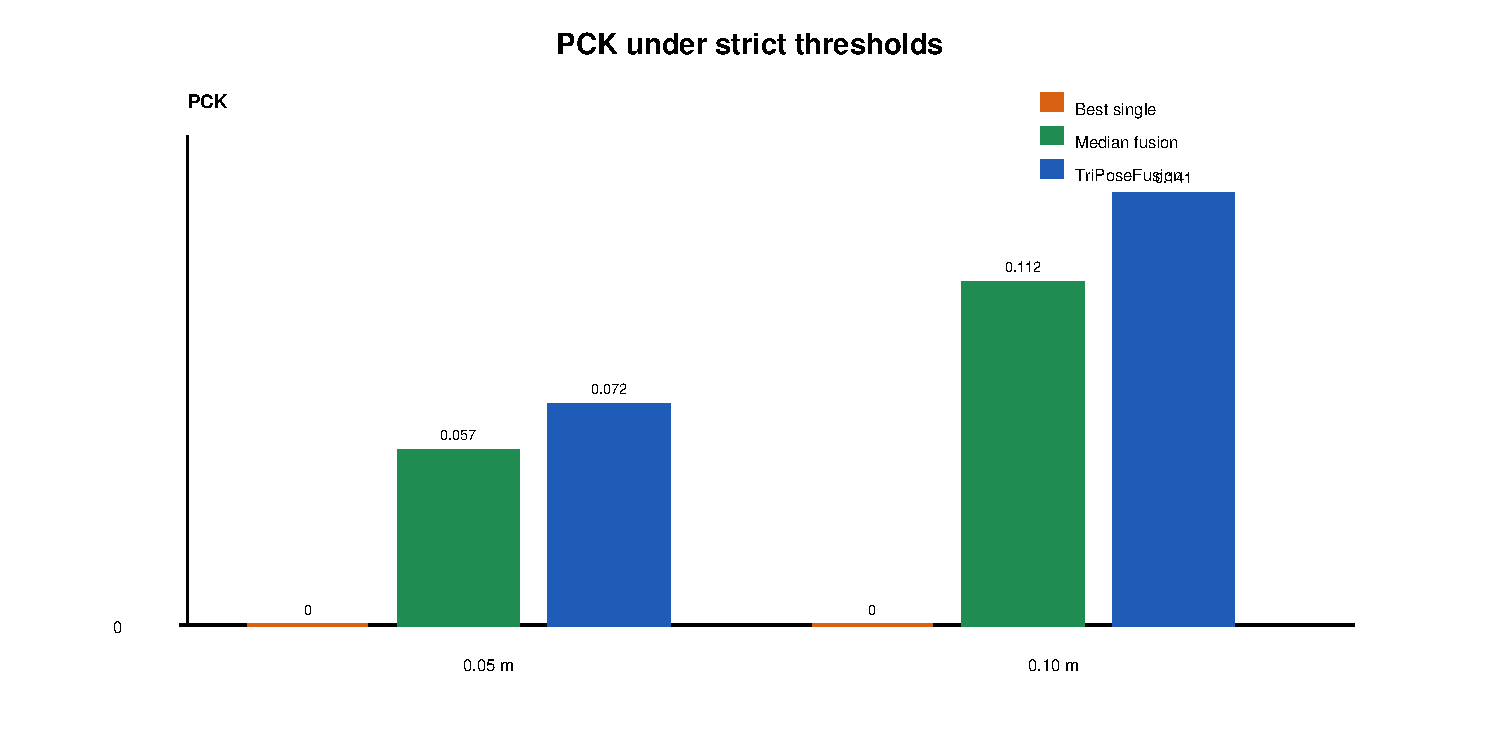
\includegraphics[width=0.76\linewidth]{figures/fig_pck_thresholds.pdf}
\caption{PCK as a function of the distance threshold. This diagnostic complements the strict PCK@0.10 value reported in the main paper and shows the threshold sensitivity of the noisy upper-body and hand-focused pseudo-reference setting.}
\label{fig:supp_pck_thresholds}
\end{figure}

\section{Diagnostic Ablations}

Table~\ref{tab:supp_twoview} reports two-view diagnostic variants. These rows were kept out of the main paper because they are auxiliary diagnostics and the left+right variant has substantially different valid/skipped coverage. The results suggest that side views can be highly informative, but the coverage mismatch means the rows should not be read as direct replacements for the full three-view setting.

\begin{table}[H]
\centering
\caption{Two-view diagnostic ablations. MPJPE and PA-MPJPE are reported in meters. Valid and Skipped denote evaluated or skipped temporal chunks.}
\label{tab:supp_twoview}
\scriptsize
\setlength{\tabcolsep}{3pt}
\begin{tabular}{lccccc}
\hline
Configuration & MPJPE (m) $\downarrow$ & PA (m) $\downarrow$ & PCK@0.10 $\uparrow$ & Valid & Skipped \\
\hline
Full three-view model & 0.412 & 0.275 & 0.141 & 21847 & 89 \\
Full two-view front+left & 0.411 & 0.273 & 0.141 & 21846 & 89 \\
Full two-view front+right & 0.415 & 0.279 & 0.141 & 21847 & 89 \\
Full two-view left+right & \textbf{0.399} & \textbf{0.255} & \textbf{0.141} & 20974 & 1506 \\
\hline
\end{tabular}
\end{table}

Table~\ref{tab:supp_diagnostic_ablation} reports additional diagnostic ablations for attention, gate weighting, and temporal refinement. These rows are separated from the main paper because they come from updated diagnostic logs with different valid-chunk coverage.

\begin{table}[H]
\centering
\caption{Additional diagnostic ablations. MPJPE and PA-MPJPE are reported in meters. Valid and Skipped denote evaluated or skipped temporal chunks.}
\label{tab:supp_diagnostic_ablation}
\scriptsize
\setlength{\tabcolsep}{3pt}
\begin{tabular}{lccccc}
\hline
Configuration & MPJPE (m) $\downarrow$ & PA (m) $\downarrow$ & PCK@0.10 $\uparrow$ & Valid & Skipped \\
\hline
Full three-view model & 0.412 & 0.275 & 0.141 & 21847 & 89 \\
No cross-view attention & 0.452 & 0.358 & 0.109 & 20424 & 88 \\
Uniform gate & 0.451 & 0.355 & 0.108 & 20424 & 88 \\
Gate only, no TCN & 0.452 & 0.358 & 0.108 & 20424 & 88 \\
\hline
\end{tabular}
\end{table}

\begin{figure}[H]
\centering
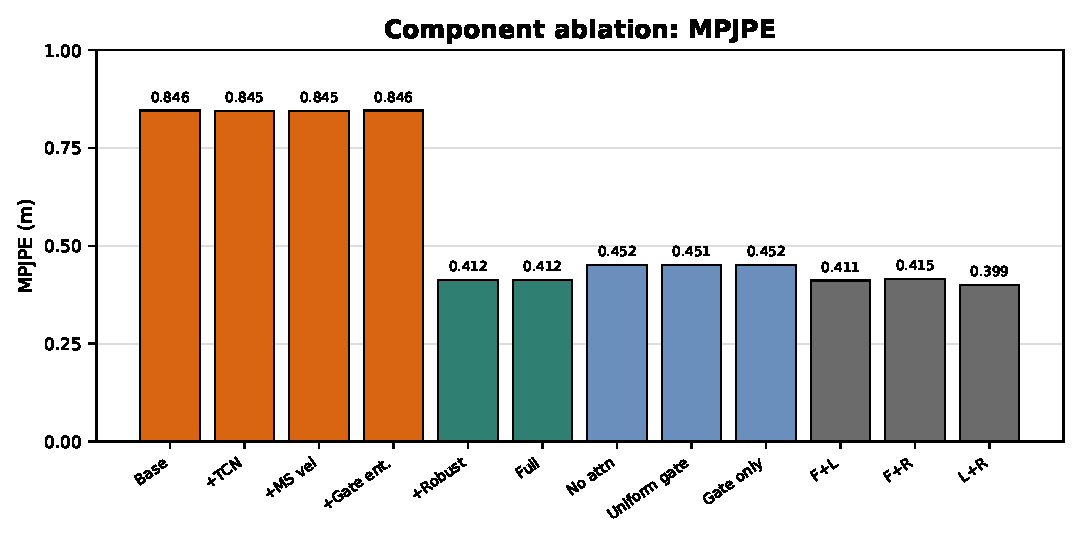
\includegraphics[width=0.72\linewidth]{figures/fig_ablation_mpjpe.pdf}
\caption{Ablation MPJPE visualization. The largest improvement comes from robust body-centered canonicalization, while temporal and gating components provide smaller secondary effects under the reported pseudo-ground-truth protocol.}
\label{fig:supp_ablation_mpjpe}
\end{figure}

\section{Gate-Weight Tables}

Table~\ref{tab:supp_gate_weights} summarizes the joint-wise gate weights corresponding to the gate discussion in the main paper. Across the 52 joints, all three views remain within $5\times10^{-5}$ of the uniform value $1/3$, supporting the interpretation that the primary gain comes from robust canonicalization rather than strong average view selection. Table~\ref{tab:supp_joint_gate_weights} reports the per-joint fusion gate values that were previously visualized as a figure.

\begin{table}[H]
\centering
\caption{Summary statistics of learned joint-wise gate weights across the 52-keypoint model space. The final column reports the maximum absolute deviation from uniform weighting ($1/3$).}
\label{tab:supp_gate_weights}
\scriptsize
\setlength{\tabcolsep}{5pt}
\begin{tabular}{lccccc}
\hline
View & Mean & Std. & Min & Max & Max $|w-1/3|$ \\
\hline
Front & 0.333344 & 0.000019 & 0.333316 & 0.333382 & 0.000049 \\
Left & 0.333339 & 0.000020 & 0.333313 & 0.333378 & 0.000045 \\
Right & 0.333350 & 0.000017 & 0.333323 & 0.333379 & 0.000045 \\
\hline
\end{tabular}
\end{table}

\begin{table}[H]
\centering
\caption{Joint-wise fusion gate weights for the front, left, and right views. Names follow the SAM3D Body MHR70 metadata after applying the 52-keypoint subset used throughout the paper.}
\label{tab:supp_joint_gate_weights}
\tiny
\setlength{\tabcolsep}{2pt}
\resizebox{\linewidth}{!}{%
\begin{tabular}{clcccclccc}
\hline
Joint & Name & Front & Left & Right & Joint & Name & Front & Left & Right \\
\hline
0 & nose & 0.333382 & 0.333377 & 0.333378 & 26 & right\_pinky\_finger\_third\_joint & 0.333334 & 0.333331 & 0.333351 \\
1 & left\_eye & 0.333381 & 0.333377 & 0.333379 & 27 & right\_wrist & 0.333340 & 0.333339 & 0.333354 \\
2 & right\_eye & 0.333382 & 0.333377 & 0.333378 & 28 & left\_thumb4 & 0.333331 & 0.333325 & 0.333335 \\
3 & left\_ear & 0.333380 & 0.333378 & 0.333378 & 29 & left\_thumb3 & 0.333331 & 0.333324 & 0.333334 \\
4 & right\_ear & 0.333381 & 0.333378 & 0.333378 & 30 & left\_thumb2 & 0.333334 & 0.333327 & 0.333335 \\
5 & left\_shoulder & 0.333379 & 0.333378 & 0.333378 & 31 & left\_thumb\_third\_joint & 0.333348 & 0.333340 & 0.333348 \\
6 & right\_shoulder & 0.333378 & 0.333378 & 0.333378 & 32 & left\_forefinger4 & 0.333342 & 0.333335 & 0.333349 \\
7 & right\_thumb4 & 0.333317 & 0.333313 & 0.333324 & 33 & left\_forefinger3 & 0.333335 & 0.333328 & 0.333340 \\
8 & right\_thumb3 & 0.333316 & 0.333313 & 0.333323 & 34 & left\_forefinger2 & 0.333330 & 0.333324 & 0.333333 \\
9 & right\_thumb2 & 0.333318 & 0.333316 & 0.333326 & 35 & left\_forefinger\_third\_joint & 0.333329 & 0.333323 & 0.333331 \\
10 & right\_thumb\_third\_joint & 0.333326 & 0.333324 & 0.333337 & 36 & left\_middle\_finger4 & 0.333348 & 0.333335 & 0.333347 \\
11 & right\_forefinger4 & 0.333322 & 0.333321 & 0.333336 & 37 & left\_middle\_finger3 & 0.333348 & 0.333337 & 0.333350 \\
12 & right\_forefinger3 & 0.333321 & 0.333320 & 0.333333 & 38 & left\_middle\_finger2 & 0.333349 & 0.333341 & 0.333353 \\
13 & right\_forefinger2 & 0.333319 & 0.333318 & 0.333331 & 39 & left\_middle\_finger\_third\_joint & 0.333340 & 0.333333 & 0.333341 \\
14 & right\_forefinger\_third\_joint & 0.333317 & 0.333315 & 0.333326 & 40 & left\_ring\_finger4 & 0.333347 & 0.333333 & 0.333346 \\
15 & right\_middle\_finger4 & 0.333343 & 0.333338 & 0.333358 & 41 & left\_ring\_finger3 & 0.333348 & 0.333334 & 0.333346 \\
16 & right\_middle\_finger3 & 0.333341 & 0.333338 & 0.333357 & 42 & left\_ring\_finger2 & 0.333349 & 0.333337 & 0.333349 \\
17 & right\_middle\_finger2 & 0.333336 & 0.333336 & 0.333353 & 43 & left\_ring\_finger\_third\_joint & 0.333348 & 0.333338 & 0.333347 \\
18 & right\_middle\_finger\_third\_joint & 0.333325 & 0.333325 & 0.333338 & 44 & left\_pinky\_finger4 & 0.333342 & 0.333320 & 0.333338 \\
19 & right\_ring\_finger4 & 0.333340 & 0.333338 & 0.333357 & 45 & left\_pinky\_finger3 & 0.333342 & 0.333323 & 0.333340 \\
20 & right\_ring\_finger3 & 0.333340 & 0.333339 & 0.333358 & 46 & left\_pinky\_finger2 & 0.333344 & 0.333328 & 0.333343 \\
21 & right\_ring\_finger2 & 0.333340 & 0.333340 & 0.333359 & 47 & left\_pinky\_finger\_third\_joint & 0.333345 & 0.333330 & 0.333342 \\
22 & right\_ring\_finger\_third\_joint & 0.333340 & 0.333340 & 0.333356 & 48 & left\_wrist & 0.333344 & 0.333329 & 0.333340 \\
23 & right\_pinky\_finger4 & 0.333333 & 0.333328 & 0.333353 & 49 & left\_acromion & 0.333379 & 0.333378 & 0.333378 \\
24 & right\_pinky\_finger3 & 0.333333 & 0.333329 & 0.333353 & 50 & right\_acromion & 0.333379 & 0.333378 & 0.333378 \\
25 & right\_pinky\_finger2 & 0.333333 & 0.333330 & 0.333353 & 51 & neck & 0.333379 & 0.333378 & 0.333378 \\
\hline
\end{tabular}
}
\end{table}

\end{document}
